\documentclass[10pt,twocolumn,letterpaper]{article}
\usepackage{cvpr}

% Include other packages here, before hyperref.
\usepackage{graphicx}
\usepackage{amsmath}
\usepackage{amssymb}
\usepackage{booktabs}
\usepackage[dvipsnames]{xcolor}
%\usepackage[belowskip=0pt,aboveskip=5pt]{caption}
\setlength{\textfloatsep}{10pt}

% If you comment hyperref and then uncomment it, you should delete
% egpaper.aux before re-running latex.  (Or just hit 'q' on the first latex
% run, let it finish, and you should be clear).
\usepackage[pagebackref,breaklinks,colorlinks,bookmarks=false]{hyperref}

% Support for easy cross-referencing
\usepackage[capitalize]{cleveref}
\crefname{section}{Sec.}{Secs.}
\Crefname{section}{Section}{Sections}
\Crefname{table}{Table}{Tables}
\crefname{table}{Tab.}{Tabs.}

% If you wish to avoid re-using figure, table, and equation numbers from
% the main paper, please uncomment the following and change the numbers
% appropriately.
%\setcounter{figure}{2}
%\setcounter{table}{1}
%\setcounter{equation}{2}

% If you wish to avoid re-using reference numbers from the main paper,
% please uncomment the following and change the counter for `enumiv' to
% the number of references you have in the main paper (here, 6).
%\let\oldthebibliography=\thebibliography
%\let\oldendthebibliography=\endthebibliography
%\renewenvironment{thebibliography}[1]{%
%     \oldthebibliography{#1}%
%     \setcounter{enumiv}{6}%
%}{\oldendthebibliography}


%%%%%%%%% PAPER ID  - PLEASE UPDATE
\def\cvprPaperID{8360} % *** Enter the CVPR Paper ID here
\def\confName{CVPR}
\def\confYear{2022}

\newcommand{\ra}{\textcolor{Periwinkle}{R1}}
\newcommand{\rb}{\textcolor{PineGreen}{R2}}
\newcommand{\rc}{\textcolor{YellowGreen}{R3}}

\newcommand{\myfirstpara}[1]{\noindent \textbf{\textit{#1:}}}
\newcommand{\mypara}[1]{\vspace{0.1em} \myfirstpara{#1}}

\newcommand{\beginsupplement}{%
        \setcounter{table}{0}
        \renewcommand{\thetable}{S\arabic{table}}%
        \setcounter{figure}{0}
        \renewcommand{\thefigure}{S\arabic{figure}}%
     }

\begin{document}

%%%%%%%%% TITLE - PLEASE UPDATE
\title{Surpassing the Human Accuracy: \\ Detecting Gallbladder Cancer from USG Images with Curriculum Learning \\ (Supplementary Material)}

\author{Soumen Basu\textsuperscript{1}, Mayank Gupta\textsuperscript{1}, Pratyaksha Rana\textsuperscript{2}, Pankaj Gupta\textsuperscript{2}, Chetan Arora\textsuperscript{1} \\
\textsuperscript{1} Indian Institute of Technology, Delhi, India \\ 
\textsuperscript{2} Postgraduate Institute of Medical Education and Research, Chandigarh, India\\
{\tt\small \href{https://gbc-iitd.github.io/gbcnet}{https://gbc-iitd.github.io/gbcnet}}
}

\maketitle

%%%%%%%%% BODY TEXT - ENTER YOUR RESPONSE BELOW
\appendix
\beginsupplement

\section{Details of Data Acquisition and Annotation}
\label{supp:data_collection}
\myfirstpara{Data Acquisition} The study was approved by the ethics committee of the Postgraduate Institute of Medical Education and Research, Chandigarh. We performed all procedures according to the Declaration of Helsinki and the research guidelines of Indian Council of Medical Research. According to the hospital's protocol, 6 hours fasting was advised a day before the Ultrasound (USG) examinations for adequate distension of the GB. Two radiologists with expertise in abdominal USG performed the examinations on a Logic S8 machine (GE Healthcare) using a convex low-frequency transducer with a frequency range of 1--5 MHz.  USG assessment was done from different angles using both subcostal and intercostal views to visualize the entire GB, including the fundus, body, and neck.  Patients were examined in different positions for adequate visualization of the GB.  The screen area was adjusted so that the GB could occupy at least 20\% of the entire screen.  

\begin{figure}[h]
    \centering
     \begin{subfigure}[b]{0.32\linewidth}
		\centering
		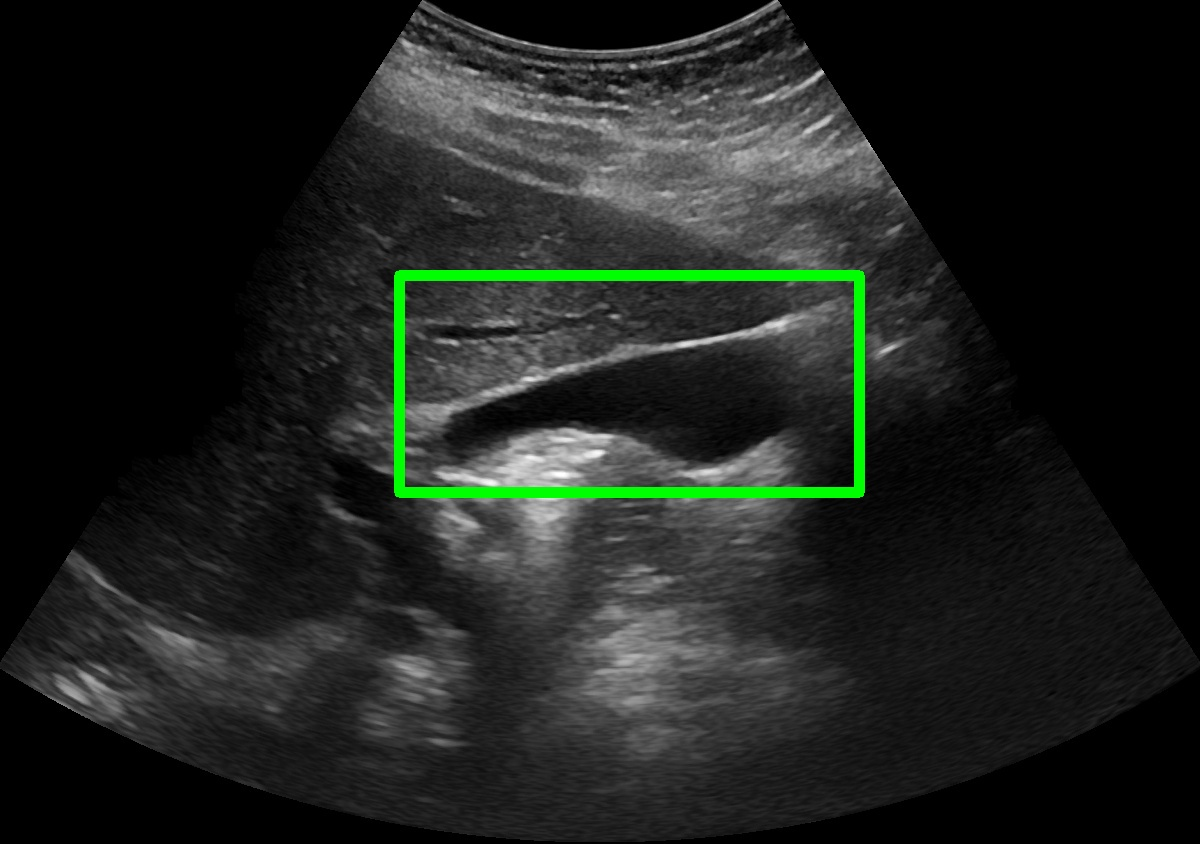
\includegraphics[width=\linewidth, height=7em]{figs/bbs-nml.png}
		\caption{}
	\end{subfigure}
    \begin{subfigure}[b]{0.32\linewidth}
		\centering
		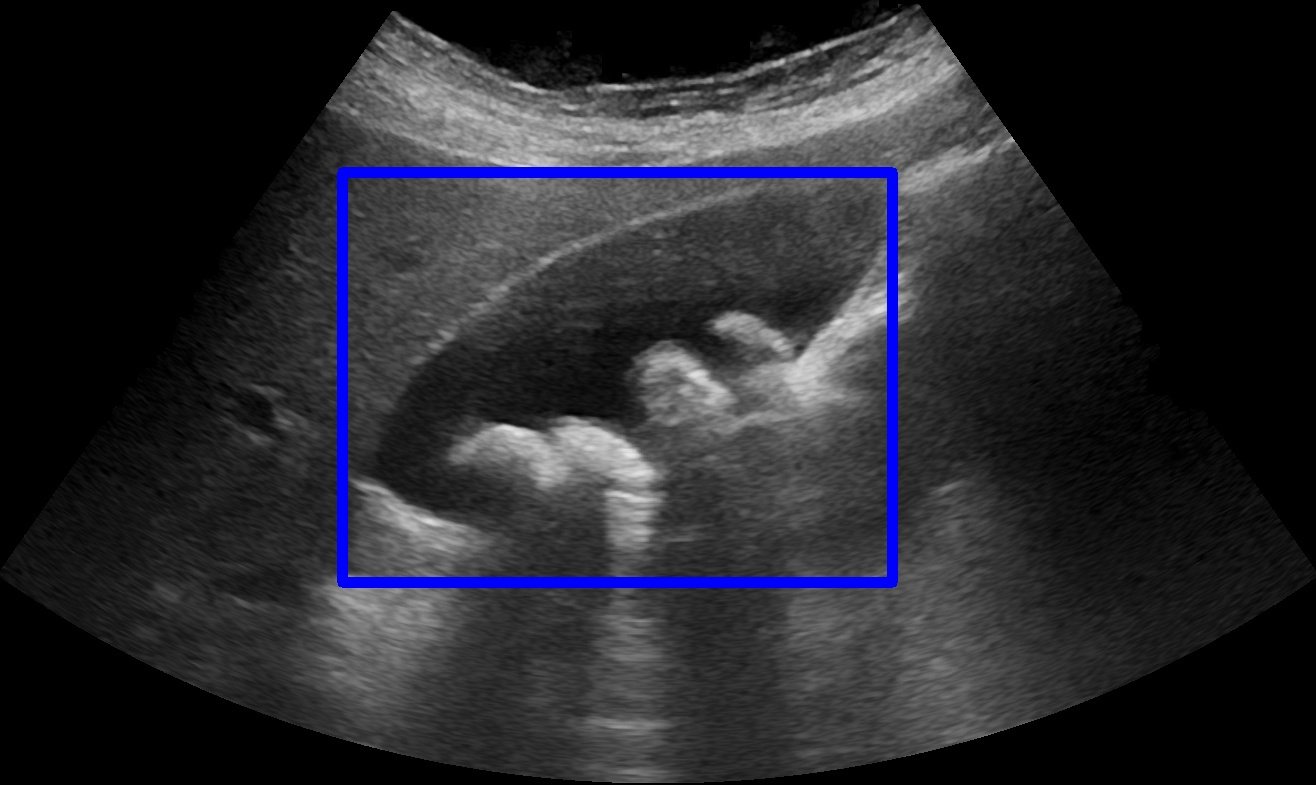
\includegraphics[width=\linewidth, height=7em]{figs/bbs-ben.png}
		\caption{}
	\end{subfigure}
    \begin{subfigure}[b]{0.32\linewidth}
		\centering
		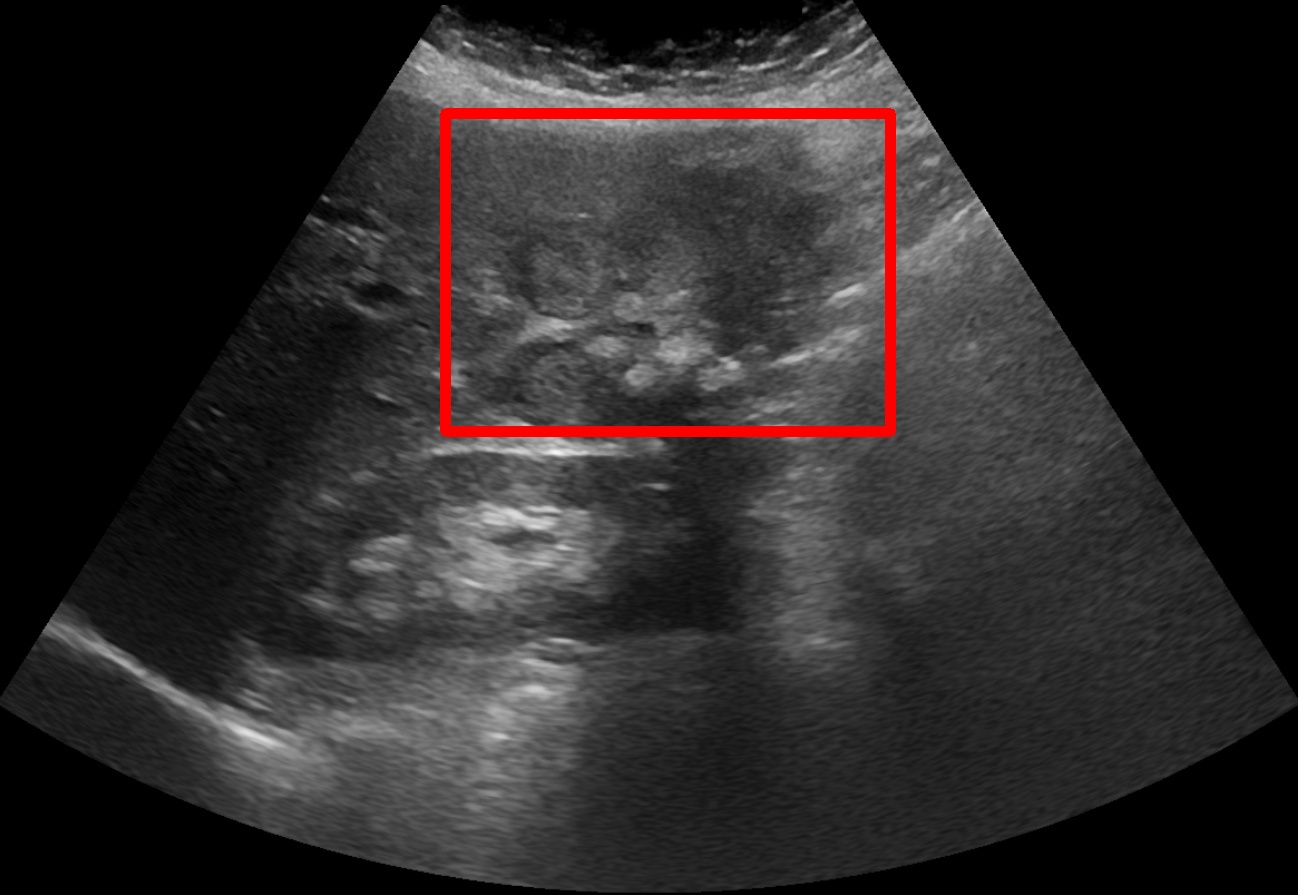
\includegraphics[width=\linewidth, height=7em]{figs/bbs-mlg.png}
		\caption{}
	\end{subfigure}
   \caption{Sample ROI annotation. (a) Normal GB with ROI annotated in green, (b) GB with benign abnormalities with ROI in blue, and (c) Malignant GB with ROI annotated in red. }
    \label{fig:bb_sample}
\end{figure}
\myfirstpara{ROI Annotation} Apart from image classification labels, we used bounding-box annotations to capture the GB localization. Two radiologists with 7 and 2 years of experience in abdomen radiology did the bounding-box annotations with consensus using the LabelMe \cite{russell2008labelme} software. A single free-size axis-aligned rectangular box in every image, spanning the entire GB and adjacent liver parenchyma, preferably keeping the GB in the box's center, highlights the region of interest (see \cref{fig:bb_sample}).


\begin{table}[t]
	\centering
	%\scriptsize
%	\captionsetup{width=\linewidth}
%    \setlength{\tabcolsep}{6pt}
	\resizebox{\linewidth}{!}{%
    \begin{tabular}{@{}lccc@{}}
    \toprule[1pt]
    \textbf{Model} & \textbf{Acc} & \textbf{Spec.} & \textbf{Sens.} \\
    \midrule[0.5pt]
    ROI+VGG16 & 53.3 $\pm$ 9.2 & 71.9 $\pm$ 11.5 & 73.3 $\pm$ 17.9\\
    ROI+VGG16+VA & 77.7 $\pm$ 4.1 & 93.8 $\pm$ 3.0 & 72.0 $\pm$ 19.5\\
    \midrule
    ROI+ResNet50 & 76.6 $\pm$ 10.7 &  82.3 $\pm$ 10.5 & 90.9 $\pm$ 11.1\\
    ROI+ResNet50+VA & 85.4 $\pm$ 7.7 & 92.3 $\pm$ 5.9 & 87.5 $\pm$ 9.1 \\
    \midrule
    ROI+Inception-V3 & 71.8 $\pm$ 8.9 & 83.3 $\pm$ 8.7 & 78.5 $\pm$ 21.4\\
    ROI+Inception-V3+VA & 82.6 $\pm$ 4.6 & 93.1 $\pm$ 4.4 & 82.6 $\pm$ 9.9\\
    \midrule
    RetinaNet & 74.9 $\pm$ 7.3 &  86.7 $\pm$ 7.8 & 79.1 $\pm$ 8.9\\
    RetinaNet+VA & 73.3 $\pm$ 6.0 & 92.1 $\pm$ 4.4 & 70.6 $\pm$ 14.2\\
    \midrule
    GBCNet (ROI+MS-SoP) & 88.2 $\pm$ 5.1 & 94.2 $\pm$ 3.7 & 92.3 $\pm$ 7.1\\
    GBCNet+VA & 92.1 $\pm$ 2.9 &  96.7 $\pm$ 2.3 & 91.9 $\pm$ 6.3\\
    \bottomrule[1pt]
    \end{tabular}
	}
	\caption{Model performances (10-fold cross-validation) for training with our proposed visual acuity-based curriculum.}
\label{tbl:curr_improve}
\end{table}

\section{Performance Improvement with Proposed Curriculum}
\label{supp:curr_improve}
We show the performance improvement of various models with the curriculum-based training in \cref{tbl:curr_improve}. All models show improvement in specificity, which indicates the effectiveness of the proposed blurring-based curriculum in tackling texture bias. 

\section{Implementation details}
%
\label{supp:impl}
\cref{tbl:configs} lists the configurations of all models which we have used. We trained on the Quadro P5000 16GB GPU. The table includes a brief description of the various stages of the network, input image sizes ($H\times W\times D$), the optimizer, relevant hyper-parameters such as learning rate, weight decay, momentum, batch size, and the number of training epochs/steps for the network. 

\begin{table*}[h]
\centering
%\scriptsize
%\setlength{\tabcolsep}{4pt}
\resizebox{ \linewidth}{!}{%
\begin{tabular}{p{0.12\linewidth}p{0.4\linewidth}p{0.06\linewidth}p{0.2\linewidth}p{0.05\linewidth}p{0.06\linewidth}}
\toprule[1.5pt]
\textbf{Model} & \textbf{Description} & \textbf{Input Size} & \textbf{Optimizer} & \textbf{Batch size} & \textbf{Epochs/ Steps}
\\ \midrule[0.75pt]
YOLOv4 \cite{yolov4} & CSPDarknet53 backbone, PANet neck, anchor-based YOLO head. Total 162-layers. Backbone was frozen for first 800 step. Entire network was trainable thereafter. Single stage, anchor-based  & $608\times608\times3$ & SGD LR = 0.0001 momentum = 0.95 weight decay = 0.0005 & 64 & 3000 steps \\ \hline
Faster-RCNN \cite{fasterrcnn} & Resnet50 Feature Pyramid backbone. Backbone was frozen for training. Two-stage, anchor-based. & $800 \times 1333 \times 3$ & SGD LR = 0.005 momentum = 0.9 weight decay = 0.0005 & 16 & 60 epochs \\ \hline
Reppoints \cite{reppoints} & Resnet101 backbone, Group Normalization neck, and a reppoints head. Backbone was frozen for first 30 epochs, and entire network was trainable thereafter. Two-stage, anchor-free & $800 \times 1333 \times 3$ & SGD LR = 0.001 momentum = 0.9 weight decay = 0.0001 & 4 & 50 epochs \\ \hline
Centripetal-Net \cite{centripetalnet} & Improvement over CornerNet model. Uses centripetal shift to match corners. HourglassNet-104 backbone. Enitre network was trainable. Anchor-free & $511 \times 511 \times 3$ & Adam LR = 0.0005 & 4 & 50 epochs \\ \hline
ResNet \cite{resnet} & Resnet-50 used. All layers were trainable. Output dimension of last fully connected layer is three - corresponding to normal, benign, and malignant GB. LR decays by 10\% after every 5 epochs through a step LR scheduler. & $224\times224\times3$ & SGD LR = 0.005 momentum = 0.9 weight decay = 0.0005 & 16 & 100 epochs \\ \hline
VGG \cite{vgg} & VGG-16 is used. All layers were trainable. LR decays by 10\% after every 5 epochs through a step LR scheduler. & $224\times224\times3$ & SGD LR = 0.005 momentum = 0.9 weight decay = 0.0005 & 16 & 100 epochs \\ \hline
Inception \cite{inception} & Inception-V3 used. All layers were trainable. LR decays by 10\% after every 5 epochs through a step LR scheduler. & $299\times299\times3$ & SGD LR = 0.005 momentum = 0.9 weight decay = 0.0005 & 16 & 100 epochs \\ \hline
RetinaNet \cite{retinanet} & Resnet-18-FPN used as backbone. All layers were trainable. Three output classes corresponding to normal, benign, and malignant GB. & $512\times512\times3$ & Adam LR = 0.0001 & 8 & 50 epochs \\ \hline
EfficientDet \cite{efficientdet} & EfficientNet-B4 used as backbone and BiFPN as feature network. All layers were trainable. Three output classes corresponding to normal, benign, and malignant GB. & $1024\times1024\times3$ & Adam LR = 0.001 & 2 & 50 epochs \\ \hline
MS-SoP Classifier (Ours) & 16 MS-SoP layers. All layers were trainable. Three output classes corresponding to normal, benign, and malignant GB. & $224\times224\times3$ & SGD LR = 0.005 momentum = 0.9 weight decay = 0.0005 & 16 & 100 epochs \\
\bottomrule
\end{tabular}
}
\caption{Implementation details for the different baseline networks used for classification and gallbladder localization.}
\label{tbl:configs}
\end{table*}

\section{Calculating Precision and Recall for GB Localization Networks}
\label{supp:eval_metric}
For computing precision and recall during the GB localization phase, as suggested by \cite{ribli2018detecting}, if the center of the predicted region lies within the bounding box of the ground truth region, then we consider a region prediction to be a true positive; otherwise, we consider the region prediction to be a false positive due to localization error. Further, we consider the zero/no region prediction as a false negative (all our images contain GB, and the localization network's task is to merely localize it). 

\section{GradCAM Visuals for GBCNet}
\label{supp:cam_vis}
Figure \ref{fig:supple-2} shows the sample Grad-CAM visualizations of the predictions using GBCNet (ROI+MS-SoP) with curriculum learning. %The blue regions show the most vital regions used by the classifier during prediction. The classifier well emphasized the crucial visual cues during inference.  

\section{ROI Visuals}
\label{supp:roi_vis}
In figure \ref{fig:supple-1}, we show sample predictions of the GB region localization for different models. We also show the region of interest as perceived by the expert radiologists. The localization model is fairly accurate in capturing important regions of the USG image.

\begin{figure*}[t]
	\centering
	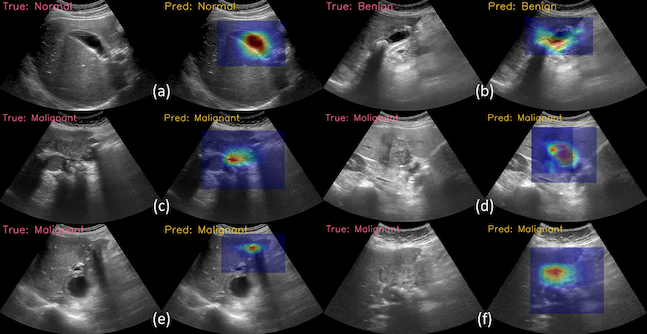
\includegraphics[width=0.9\linewidth]{figs/vis-s-1.png}
	\caption{Sample Grad-CAM visuals of GBCNet with curriculum learning. (a) Normal, (b) Benign, and (c)--(f) Malignant samples.}
	\label{fig:supple-2}
\end{figure*}

\begin{figure*}[t]
	\centering
	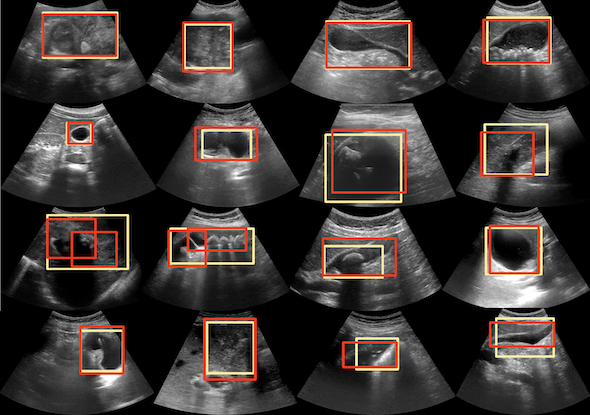
\includegraphics[width=0.9\linewidth]{figs/vis-s-0.png}
	\caption{Sample visual results of RoI Detection models. First row - Faster-CNN, second row - YOLOv4, third row - Reppoints, and fourth row - CentripetalNet. Dark red is the ROI prediction by the model and light yellow is expert radiologists' perception of ROI.}
	\label{fig:supple-1}
\end{figure*}

{\small
\bibliographystyle{ieee_fullname}
\bibliography{gbc-ref}
}

\end{document}
